\documentclass[demo, 12pt, notitlepage, letterpaper]{report}
\usepackage[version=4]{mhchem}
\usepackage{siunitx}
\usepackage[margin=1in]{geometry}
\usepackage{tabularx}
\usepackage{ragged2e}
\usepackage[font=small]{caption}
\usepackage{calculator}
\usepackage{luacode}
\usepackage{pythontex}

\DeclareSIUnit\ml{\milli\litre}
\DeclareSIUnit\mpl{\mol\per\litre}
\DeclareSIUnit\mmol{\milli\mole}
\DeclareSIUnit\gpl{\gram\per\mol}
\DeclareSIUnit\kjpmol{\kilo\joule\per\mol}
\DeclareSIUnit\heatcap{\joule\per\celsius\per\gram}

\sisetup{space-before-unit = true, free-standing-units = true}

\title{Thermokinetics Lab}
\author{Leon Si}
\date{February 22, 2022}

\begin{document}
\maketitle

% Rubric:
% Sufficient relevant quantitative and qualitative raw data supports a detailed and valid research question conclusion.
% Appropriate and sufficient data processing is carried out with the accuracy required to validate conclusion; fully consistent with the experimental data.
% Full and appropriate consideration of the impact of measurement uncertainty on the analysis.
% Processed data correctly interpreted so that a completely valid and detailed conclusion to the research question can be deduced.

\section*{Data}

% \begin{noindent}
\begin{pycode}
from sigfig import round
# Three sig fig
def tsf(num):
	return round(str(num), sigfigs = 3)
\end{pycode}
% \end{noindent}

% \begin{noindent}
\begin{pycode}
"""
[0]: Volume of CuSO4 Time of Zn Addition
[1]: Initial temp
[2]: Time of Zn addition
[3]: b value for equation of cooling line
[4]: m value for equation of cooling line (could be positive/negative)
[5]: R value of cooling line
"""

raw_data = [
	# Eric, Bobby, Bryan	20	24.4	72	75.358 - 0.0417x	-0.9918
	[20, 24.4, 72, 75.358, -0.0417, -0.9918],
	# Estelle, Hannah, Molly 	20	24.2	132	76.057 - 0.0521x	-0.9591
	[20, 24.2, 132, 76.1, -0.0521, -0.9591],
	# Lily, Cindy, Devanshi	20	24.2	60	74.909-0.086299x	-0.99338
	[20, 24.2, 60, 74.9, -0.086299, -0.99338],
	# Kevin, Leon, Thomas	20	24.8	72	38.948 - 0.0052021x	-0.95144
	[20, 24.8, 72, 38.948, -0.0052021, -0.95144],
	# Avaneesh, Artin, Ethan, Yucen	20	24.6	96	75.883 - 2.5313x	-0.99564
	[20, 24.6, 96, 75.883, -2.5313 / 60, -0.99564], # time of cooling line was given in minutes
	# Colin, Henry, Collin, Ishan	20	23.1	14	35.707+0.0060035x	0.952365476
	[20, 23.1, 14, 35.707, 0.0060035, 0.952365476],
	# Jasmine, Amy, Tina	20	23.8	15	74.526-0.059536x	-0.8973
	[20, 23.8, 15, 74.526, -0.059536, -0.8973],
	# Prachi, Michelle, Naina 	20	24.6	96	61.881 - 0.02918	-0.99694
	[20, 24.6, 96, 61.881, -0.02918, -0.99694],
]

headers = (
	'volume',
	'initial_temp',
	'zinc_addition_time',
	'cooling_line_b',
	'cooling_line_m',
	'r_value'
)

data = [
	dict(zip(headers, row)) for row in raw_data
]

def get_data_row(row_index: int):
	row = data[row_index]
	sign = "+" if row['cooling_line_m'] > 0 else "-"
	equation = f"{tsf(row['cooling_line_m'])} {sign} {tsf(abs(row['cooling_line_b']))}$x$"

	return f"""
		{row_index + 1}
		& {row['volume']}
		& {row['initial_temp']}
		& {row['zinc_addition_time']}
		& {equation}
		& {tsf(row['r_value'])}
	"""
\end{pycode}
% \end{noindent}

\begin{table}[hbt!]
	\caption{Data collected from 8 trials of the experiment. Equation of cooling line approximates the temperature of the solution in Celsius at $x$ seconds. The parameters are rounded to 3 significant figures.}
	\def\arraystretch{1.5}
	\begin{tabularx}{\linewidth}{|
			>{\RaggedRight}X|
			>{\RaggedRight}X|
			>{\RaggedRight}X|
			>{\RaggedRight}X|
			>{\RaggedRight}X|
			>{\RaggedRight}X|
		}
		\hline
		Trial \#
		 & Volume of \ce{CuSO4} /\ml
		 & Baseline temperature /\celsius
		 & Time of \ce{Zn} addition /\second
		 & Equation of cooling line
		 & R value
		\\\hline
		\py{get_data_row(0)}
		\\\hline
		\py{get_data_row(1)}
		\\\hline
		\py{get_data_row(2)}
		\\\hline
		\py{get_data_row(3)}
		\\\hline
		\py{get_data_row(4)}
		\\\hline
		\py{get_data_row(5)}
		\\\hline
		\py{get_data_row(6)}
		\\\hline
		\py{get_data_row(7)}
		\\\hline
	\end{tabularx}
\end{table}

\section*{Analysis}

The data in Table 1 can be used to find the molar enthalpy of formation of \ce{ZnSO4}. For the following calculations, the values in Trial 4 are used.

To find the molar enthalpy of formation of \ce{ZnSO4}, the energy change of the reaction $Q_{reaction}$ and the moles of \ce{ZnSO4} ($n_{ZnSO4}$) must be known.

To find the moles of \ce{ZnSO4} produced, the moles of \ce{CuSO4} must be knonwn. Using the known concentration of \ce{CuSO4} (1\mpl), the volume of \ce{CuSO4} can be converted to moles of \ce{CuSO4}:
\begin{align*}
	c     & = \frac{n}{V}        \\
	1\mpl & = \frac{n}{20\ml}    \\
	n     & = 20\mmol~\ce{CuSO4}
\end{align*}

Then, to find the moles of \ce{ZnSO4}, the balanced chemical equation of the reaction between zinc metal (\ce{Zn}) and aqueous copper sulfate (\ce{CuSO4}) is used:

\centerline{\ce{CuSO4_{(aq)} + Zn_{(s)} -> ZnSO4_{(aq)} + Cu_{(s)}}}

This equation gives the mole ratio between \ce{CuSO4} and \ce{ZnSO4}, which can be used to find the moles of \ce{ZnSO4} produced in the reaction:
\begin{align*}
	n_{\ce{ZnSO4}} & = 20\mmol~\ce{CuSO4} * \frac{1\mol~{\ce{ZnSO4}}}{1\mol~{\ce{CuSO4}}} = 20\mmol~{\ce{ZnSO4}}
\end{align*}

In addition to the number of moles of \ce{ZnSO4}, the change in energy of the reaction ($Q_{reaction}$) must also be known. The energy lost by the reaction is equal to the energy gained by the solution: $Q_{reaction} = -Q_{solution}$. To find $Q_{solution}$, the mass $m$ of the solution, the specific heat capacity $c$ of the solution, and the temperature change $\Delta T$ of the solution are all needed.

Since the solution is dilute, the mass of the solution can be approximated using the density of water, 1~\unit{\gram\per\cm}. Thus, the mass of the solution is:
\begin{align*}
	m & = \rho * V                      \\
	m & = 1~\unit{\gram\per\cm} * 20\ml \\
	m & = 20\gram
\end{align*}

The heat capacity of the solution is approximated with the specific heat capacity of water (4.184\heatcap). Thus, $c = 4.184\heatcap$

To calculate the change in temperature of the solution, the initial and final temperatures are needed. The initial temperature of the solution before the reaction ($T_i$) is equal to the \textit{Baseline temperature} column in Table 1.

To obtain the final temperature of the solution, the cooling of the solution needs to be taken into account. This is done by plugging in the time when \ce{Zn} was added into the solution into the equation of the cooling line.
\begin{align*}
	T_f & = 38.948 - 0.0052021x    \\
	T_f & = 38.948 - 0.0052021(72) \\
	T_f & = 38.5734488\celsius
\end{align*}

This value represents the point $x$ in the following graph:

\centerline{\noindent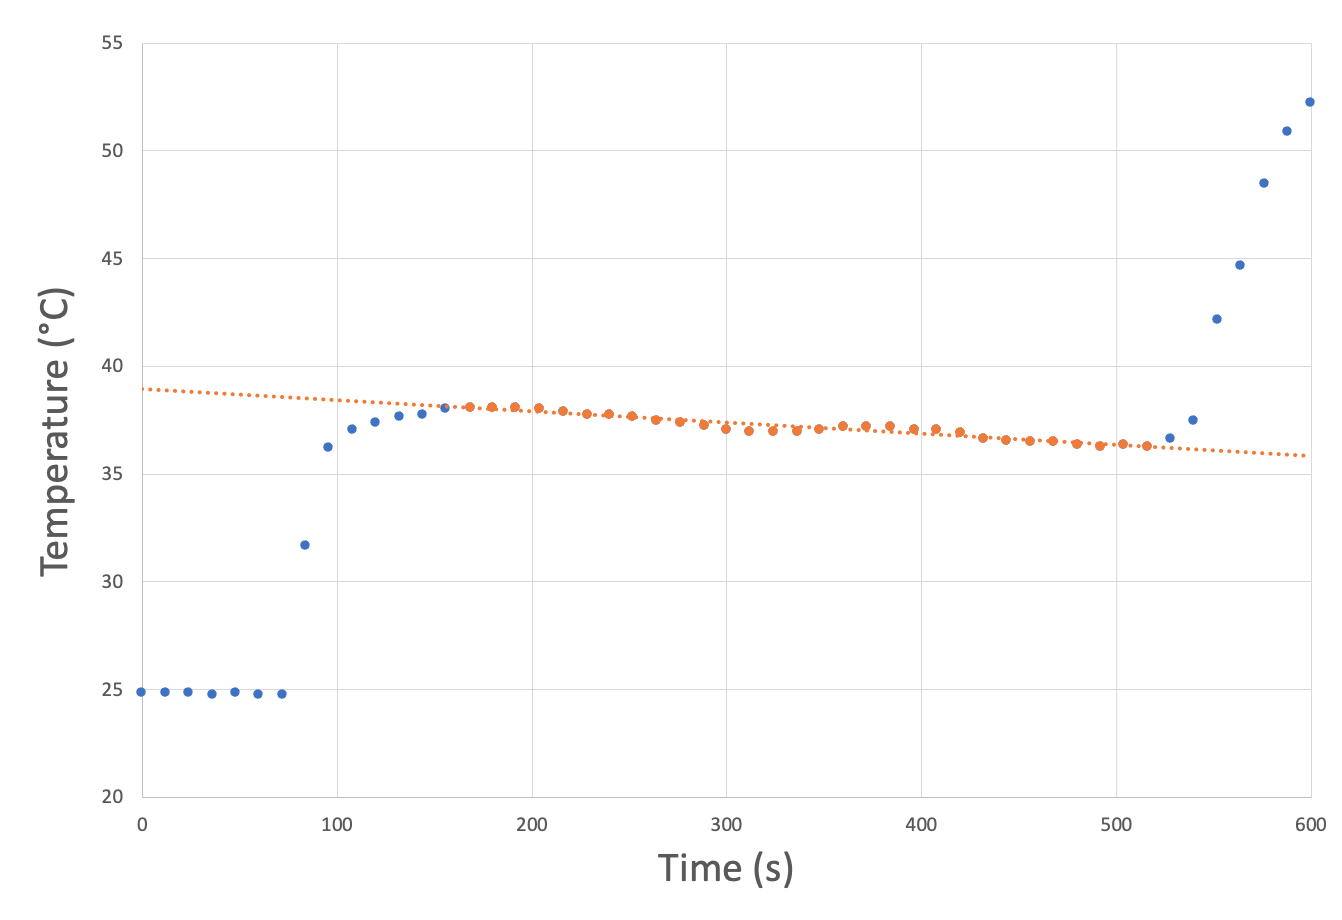
\includegraphics{time-vs-temperature.png}}

With these values, the energy change of the solution and the energy change of the reaction can be determined:
\begin{align*}
	Q_{solution} & = mc\Delta T = mc(T_f - T_i)
	\\
	Q_{solution} & = (20\gram) * (4.184\heatcap) * (38.5734\celsius - 24.8\celsius)
	\\
	Q_{solution} & = 1152.56\joule
	\\
	Q_{reaction} & = -Q_{solution}
	\\
	Q_{reaction} & = -1152.56\joule
\end{align*}

Finally, the molar enthalpy of the reaction can be calculated:
\begin{align*}
	\Delta H_{reaction} & = \frac{Q_{reaction}}{n}                        \\
	\Delta H_{reaction} & = \frac{-1152.56\joule}{0.02\mol}               \\
	\Delta H_{reaction} & = -57628~\unit{\joule\per\mol} = -57.628\kjpmol
\end{align*}

Performing the above calculation for all trials gives the following table of values:

% \begin{noindent}
\begin{pycode}
def get_final_temp(row_index: int):
	row = data[row_index]
	t_final = row['cooling_line_b'] + row['zinc_addition_time'] * row['cooling_line_m']
	return t_final

def get_q_reaction(row_index: int):
	row = data[row_index]
	m = row['volume']
	c = 4.184
	t_initial = row['initial_temp']
	t_final = get_final_temp(row_index)
	q = -1 * m * c * (t_final - t_initial)
	return q

def get_h_reaction(row_index: int):
	q = get_q_reaction(row_index)
	mols = 0.02
	h = q / mols / 1000 # kJ/mol
	return h

def get_table_2_row(row_index: int):
	row = data[row_index]
	return f"""
		{row_index + 1}
		& {tsf(get_final_temp(row_index))}
		& {tsf(get_q_reaction(row_index))}
		& {tsf(get_h_reaction(row_index))}
	"""
\end{pycode}
% \end{noindent}

\begin{table}[hbt!]
	\caption{Calculations of $\Delta H_{reaction}$ for all trials.}
	\def\arraystretch{1.5}
	\begin{tabularx}{\linewidth}{|
			p{0.1\linewidth}|
			p{0.3\linewidth}|
			>{\RaggedRight}X|
			>{\RaggedRight}X|
		}
		\hline
		Trial \#
		 & Final Temperature $T_f$ /\unit{\celsius}
		 & $Q_{reaction}$ /\unit{\joule\per\mol}
		 & $\Delta H_{reaction}$ /\unit{\kjpmol}
		\\\hline
		\py{get_table_2_row(0)}
		\\\hline
		\py{get_table_2_row(1)}
		\\\hline
		\py{get_table_2_row(2)}
		\\\hline
		\py{get_table_2_row(3)}
		\\\hline
		\py{get_table_2_row(4)}
		\\\hline
		\py{get_table_2_row(5)}
		\\\hline
		\py{get_table_2_row(6)}
		\\\hline
		\py{get_table_2_row(7)}
		\\\hline
	\end{tabularx}
\end{table}

Thus, the experimental value for $\Delta H_{reaction}$ can be determined by taking the average of the values from all 8 trials. The uncertainty can be calculated using the half-range method:

% \begin{noindent}
\begin{pycode}
h_reactions = [get_h_reaction(row_index) for row_index in range(0, len(data))]
avg_h_reaction = sum(h_reactions) / len(data)
avg_h_reaction_rounded = round(str(avg_h_reaction), sigfigs = 5)
\end{pycode}
% \end{noindent}

\begin{align*}
	\Delta H_{reaction} & = \frac{-201 + -188 + -191 + -57.6 + -198 + -53.1 + -209 + -144}{8} \\
	\Delta H_{reaction} & = \py{avg_h_reaction_rounded}\kjpmol
\end{align*}

\subsection*{Comparison with Theoretical Value}
To find the theoretical value of this reaction, the following formula is used:

\begin{align*}
	\Delta H_{reaction} = \sum \Delta {H_f}_{products} - \sum \Delta {H_f}_{reactants}
\end{align*}

% \begin{noindent}
\begin{pycode}
expected_h_reaction = -980.14 - (-769.98)
\end{pycode}
% \end{noindent}

According to NIST, the molar enthalpy formation of \ce{CuSO4} is -769.98\kjpmol and the molar enthalpy of formation of \ce{ZnSO4} is -980.14\kjpmol . Because \ce{Zn} and \ce{Cu} are in their standard states, the molar enthalpy of \ce{Zn} and \ce{Cu} is 0\kjpmol .
\begin{align*}
	\Delta H_{reaction} & = -980.14\kjpmol - (-769.98\kjpmol) \\
	\Delta H_{reaction} & = -210.16\kjpmol
\end{align*}

This theoretical value can be used to determine the percent error of the value obtained from the experimental trials:

% \begin{noindent}
\begin{pycode}
percent_error = abs((avg_h_reaction - expected_h_reaction) / expected_h_reaction)
\end{pycode}
% \end{noindent}

\begin{align*}
	\delta & = |\frac{v_A - v_E}{v_E}| * 100\%                                   \\
	\delta & = |\frac{\py{avg_h_reaction_rounded} - (-210.16)}{-210.16}| * 100\% \\
	\delta & = \py{round(percent_error * 100, sigfigs = 3)}\%
\end{align*}

However, from the experimental data, there are potentially two outliers: Trial 3 and Trial 5. Because there is potentially more than one outlier, the Dixon Q test cannot be used since it is only valid for data that has exactly one outlier. Instead, to determine these outliers in our data, the Tietjen-Moore test is used instead.

The Tietjen-Moore test calculates a test statistic $L_k$ based on the data. The value of the test statistic is between zero and one: if there are no outliers in the data, the test statistic is close to 1, and if there are outliers in the data, it will be closer to 0. For a data set with exactly $k$ outliers, the formula for calculating the test statistic $L_k$ for a Tietjen-Moore test is:
\begin{align*}
	L_k = \frac{\sum_{i=1}^{n-k}(y_i-\bar{y}_k)^2}{\sum_{i=1}^{n}(y_i-\bar{y})^2}
\end{align*}

where $n$ is the number of data points in our data set, $\bar{y}$ denotes the mean for all trials, and $\bar{y}_k$ denotes the sample mean with the largest $k$ points removed. It is suspected that there are 2 outliers in the experimental results displayed in Table 2. Thus, $k = 2$:

% \begin{noindent}
\begin{pycode}
import numpy as np
# Retrieving the data with the two largest values removed
filtered_h_reactions = sorted(h_reactions)[:-2]
full_mean = np.mean(h_reactions)
filtered_mean = np.mean(filtered_h_reactions)

numerator = sum([
	(y - filtered_mean) ** 2 for y in filtered_h_reactions
])
denominator = sum([
	(y - full_mean) ** 2 for y in h_reactions
])

L_2 = numerator / denominator
\end{pycode}
% \end{noindent}

\begin{align*}
	L_2 & = \frac{\sum_{i=1}^{8-2}(y_i-\bar{y}_2)^2}{\sum_{i=1}^{8}(y_i-\bar{y})^2} \\
	L_2 & = \py{tsf(L_2)}
\end{align*}

Because this test statistic is close to zero, it strongly suggests that there are two outliers in the data. Removing these outliers (Trial 3 and Trial 5) from our data and recalculating the $\Delta H_{reaction}$ gives a much smaller percent error:

% \begin{noindent}
\begin{pycode}
avg_h_reaction_2 = np.mean(filtered_h_reactions)
avg_h_reaction_2_rounded = round(str(avg_h_reaction_2), sigfigs = 5)
percent_error_2 = abs(
	(avg_h_reaction_2 - expected_h_reaction) / expected_h_reaction
)
\end{pycode}
% \end{noindent}

\begin{align*}
	\Delta {H_{reaction}}_{2} & = \frac{-201 + -188 + -191 + -198 + -209 + -144}{6}                   \\
	\Delta {H_{reaction}}_{2} & = \py{avg_h_reaction_2_rounded}\kjpmol                                \\
	\delta                    & = |\frac{\py{avg_h_reaction_2_rounded} - (-210.16)}{-210.16}| * 100\% \\
	\delta                    & = \py{round(percent_error_2 * 100, sigfigs = 3)}\%
\end{align*}

\section*{Conclusion}

% Presentation of the investigation is clear. Errors do not hamper understanding of the focus, process and outcomes.
% Clear report structure; necessary information on focus, process and outcomes is present and presented coherently.
% Report is relevant and concise; facilitates a ready understanding of the focus, process and outcomes.
% Subject specific terminology and conventions is appropriate and correct. Errors do not hamper understanding.
\end{document}
